% !TeX root = main.tex
%\documentclass[12pt,xcolor={dvipsnames}]{beamer}
\documentclass{beamer}
\beamerdefaultoverlayspecification{<+->}

%\usepackage[usenames,dvipsnames]{xcolor}
\definecolor{mynicegreen}{RGB}{0, 111, 0}
\usefonttheme{professionalfonts} % using non standard fonts for beamer
\usefonttheme{serif}
%\usepackage{euler}
\usepackage{hyperref}
\newcommand{\Rm}{\mathrm{Rm}}
\newcommand{\om}{\mathbb{M}}
\newcommand{\KN}{\mathbin{\bigcirc\mspace{-15mu}\wedge\mspace{4mu}}}
\newcommand{\Ric}{\mathrm{Ric}}
\newcommand{\Scal}{\mathrm{Scal}}
\newcommand{\mm}{\mathcal{M}}
\newcommand{\RICC}{{\sf RICC}}
\newcommand{\SC}{{\sf SC}}
\newcommand{\nn}{\mathcal{N}}
\renewcommand{\iint}{\mathrm{int}}
\newcommand{\MYhref}[3][magenta]{\href{#2}{\color{#1}{#3}}}      
\newcommand{\parent}[1]{\left( #1 \right)}


\newcommand{\V}{\mathbb{V}}
\newcommand{\divv}{\operatorname{div}}
\newcommand{\tr}{\mathrm{tr}}
\newcommand{\dv}{\operatorname{dVol}_g}
\newcommand{\ddv}{\widetilde{\operatorname{dVol}_g}}
\newcommand{\End}{\operatorname{End}}
\newcommand{\dx}{\mathrm{d}x}
\newcommand{\dr}{\mathrm{d}r}
\newcommand{\R}{\mathscr{R}}
\newcommand{\n}{\nabla}
\newcommand{\W}{\mathscr{W}}
\newcommand{\Sy}{\mathcal{S}}
\newcommand{\T}{\mathscr{T}}
\newcommand{\Endo}{\operatorname{End}}
\newcommand{\w}{\omega}
\newcommand{\signature}{\Sigma}             %The signature set.
\newcommand{\Id}{\mathrm{Id}}
\newcommand{\ee}{\mathcal{E}}
\newcommand{\sop}{\mathcal{S}}
\newcommand{\be}{\mathbf{e}}
\newcommand{\ww}{\mathcal{W}}



\newtheorem{perg}{Pergunta}
\newcommand{\quotes}[1]{``#1''}
\usepackage{changepage}
\date{33 de fevereiro de 2222}
%\usepackage{newpxtext,eulerpx}

% The Beamer class comes with a number of default slide themes
% which change the colors and layouts of slides. Below this is a list
% of all the themes, uncomment each in turn to see what they look like.

%\usetheme{default}
%\usetheme{AnnArbor}
%\usetheme{Antibes}
%\usetheme{Bergen}
%\usetheme{Berkeley}
%\usetheme{Berlin}
%\usetheme{Boadilla}
%\usetheme{CambridgeUS}
%\usetheme{Copenhagen}
%\usetheme{Darmstadt}
%usetheme{Dresden}
%\usetheme{Frankfurt}
%\usetheme{Goettingen}
%\usetheme{Hannover}
%\usetheme{Ilmenau}
%\usetheme{JuanLesPins}
%\usetheme{Luebeck}
\usetheme{Madrid}
\colorlet{beamer@blendedblue}{blue!40!black}
%\usetheme{Malmoe}
%\usetheme{Marburg}
%\usetheme{Montpellier}
%\usetheme{PaloAlto}
%\usetheme{Pittsburgh}
%\usetheme{Rochester}
%\usetheme{Singapore}
%\usetheme{Szeged}
%\usetheme{Warsaw}

% As well as themes, the Beamer class has a number of color themes
% for any slide theme. Uncomment each of these in turn to see how it
% changes the colors of your current slide theme.

%\usecolortheme{albatross}
%\usecolortheme{beaver}
%\usecolortheme{beetle}
%\usecolortheme{crane}
%\usecolortheme{dolphin}
%\usecolortheme{dove}
%\usecolortheme{fly}
%\usecolortheme{lily}
%\usecolortheme{orchid}
%\usecolortheme{rose}
%\usecolortheme{seagull}
%\usecolortheme{seahorse}
%\usecolortheme{whale}
%\usecolortheme{wolverine}

%\setbeamertemplate{footline} % To remove the footer line in all slides uncomment this line
%\setbeamertemplate{footline}[page number] % To replace the footer line in all slides with a simple slide count uncomment this line

\setbeamertemplate{navigation symbols}{} % To remove the navigation symbols from the bottom of all slides uncomment this line
\usepackage[brazilian]{babel}
\usepackage{mathrsfs}
\usepackage[utf8]{inputenc}
%\usepackage[T1]{fontenc}
%\usepackage{mathpple}
%\usepackage[euler-digits]{eulervm}
\usepackage{lmodern}
\usepackage{lipsum}  
%\usepackage[sc]{mathpazo}
%\linespread{1.05} 
%\usepackage[osf,sc]{mathpazo}
\usepackage{graphicx} % Allows including images
\usepackage{booktabs} % Allows the use of \toprule, \midrule and \bottomrule in tables
\DeclareMathOperator{\sen}{sen}
\DeclareMathOperator{\senh}{senh}





%----------------------------------------------------------------------------------------
%	TITLE PAGE
%----------------------------------------------------------------------------------------

\title[Apresentação sobre...]{Insira o título da apresentação aqui} % The short title appears at the bottom of every slide, the full title is only on the title page

\author[Neumann, V.]{
\includegraphics[width=0.8\textwidth]{unb.eps} \\  \[ \begin{aligned}
&\textbf{Aluno:} \text{ Insira o seu nome aqui} \\
&\textbf{Orientador:} \text{ preencha aqui (ou comente essa linha)} \\
\end{aligned}
\] }

   

\begin{document}

\begin{frame}
\titlepage % Print the title page as the first slide
\end{frame}



%----------------------------------------------------------------------------------------
%	PRESENTATION SLIDES
%----------------------------------------------------------------------------------------


%------------------------------------------------

\begin{frame}
\frametitle{Eratóstenes: o homem que mediu o mundo}
\begin{figure}[H]
\centering
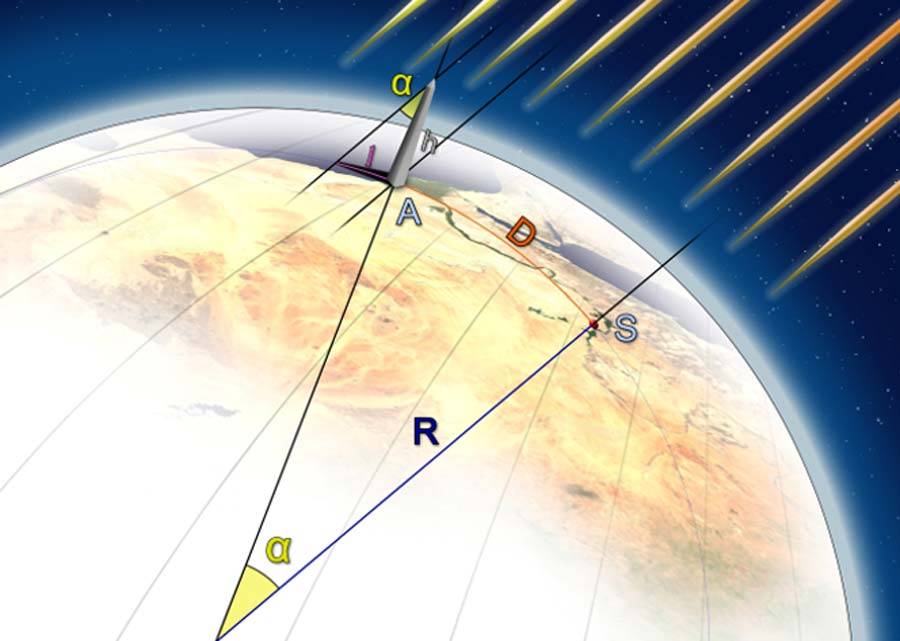
\includegraphics[scale=.35]{./IMAGES/erast.jpg}
\end{figure}
\end{frame}



\begin{frame}
\frametitle{Conceitos e notações preliminares}
\begin{itemize}
\item Uma variedade fechada é uma variedade compacta e sem bordo. 
\item Todas as variedades com as quais trabalharemos são, por hipótese, conexas e sem bordo.
\item Uma vez fixada uma variedade Riemanniana $\parent{\mm^n, g}$, denotaremos por $\T^{k}_{\ell}\parent{T \mm}$ o fibrado de tensores de tipo $(k, \ell)$ sobre $\mm$. 
\item $\Lambda^k\parent{\mm} \subset \T^0_k\parent{T \mm}$ denota o fibrado de $k$-formas diferenciáveis sobre $\mm$. 
\item O operador estrela de Hodge será denotado por $$\star: \Lambda^k\parent{ \mm} \to \Lambda^{n-k}\parent{\mm}.$$
\item Os isomorfismos musicais bemol e sustenido serão denotados, respectivamente, por $\flat$ e $\sharp$. Não explicitaremos as identificações fornecidas por tais aplicações.
\iffalse
\item Seja $(\mm^n, g)$ uma variedade Riemanniana e fixe $\{\be_1, \ldots, \be_n \}$ um referencial local $g$-ortonormal definido num aberto $U \subset \mm$, sendo $\{\be^1, \ldots, \be^n\}$ o co-referencial associado (determinado por $\be^i(\be_j) = \delta^i_j$).
\fi 
\end{itemize}
\end{frame}

\begin{frame}
\frametitle{Conceitos e notações preliminares}
\begin{itemize}
\item A manifestação de um tensor $P \in \T^{0}_4\parent{ T \mm}$ de tipo curvatura como um endomorfismo auto-adjunto de $\Lambda^2\parent{\mm}$ é caracterizada por
\[
P\parent{X \wedge Y} = \sharp\parent{P\parent{X \wedge Y, \bullet}},
\]
sejam quais forem $X, Y \in \Gamma\parent{T \mm}$. 
\item $\KN: \T^{0}_2(T \mm) \times \T^{0}_2(T \mm)\to \T^{0}_4(T \mm)$ denotará o produto de Kulkarni-Nomizu, determinado por
\[  \begin{aligned} 2 \cdot (T \KN S)(X, Y, Z, W) &= T(Y, Z) S(X, W) - T(X, Z) S(Y, W) \\ 
&+ S(Y, Z) T(X, W) - S(X, Z) T(Y, W),
\end{aligned}
 \]
sejam quais forem $X, Y, Z, W \in \Gamma\parent{T \mm}$.
\end{itemize}
\end{frame}

\begin{frame}
\frametitle{Conceitos e notações preliminares}
\begin{itemize}
\item O tensor de Einstein de $\mm$, a saber,
\[
E \doteq \Ric - \frac{\Scal}{n} g
\] será denotado por $E$.
\end{itemize}
\end{frame}

\begin{frame}
\frametitle{Sumário} % Table of contents slide, comment this block out to remove it
\tableofcontents % Throughout your presentation, if you choose to use \section{} and \subsection{} commands, these will automatically be printed on this slide as an overview of your presentation
\end{frame}


\section{Prólogo}
\begin{frame}
\frametitle{Os primórdios}
Entender as relações entre topologia e curvatura tem sido, desde sempre, uma das áreas de pesquisa mais ativas em geometria. Nesse sentido, dois problemas antigos e muito populares, são:
\begin{perg}
Quais são todas as topologias possíveis de uma superfície fechada?
\end{perg}
\begin{perg}
Qual é a \quotes{melhor} métrica que uma superfície fechada qualquer admite?
\end{perg}
\pause
Veremos que essas duas questões estão intimamente relacionadas. 
\end{frame}
\begin{frame}
\frametitle{Dimensão 2: superfícies}
Em dimensão $2$, a topologia é bem entendida e caracterizada pela seguinte:
\begin{block}{A classificação de superfícies fechadas}
\textit{Toda variedade bi-dimensional $\mm^2$ conexa e fechada é homeomorfa a exatamente um dos seguintes espaços:
\begin{itemize}
\item a esfera $\mathbb{S}^2$;
\item a soma conexa finita de uma ou mais cópias do toro $\mathbb{T}^2 = \mathbb{S}^1 \times \mathbb{S}^1$;
\item a soma conexa finita de uma ou mais cópias do plano projetivo $\mathbb{R}\mathbb{P}^2$.
\end{itemize}
}
\end{block}
\end{frame}

\begin{frame}
\frametitle{Dimensão 2: superfícies}
\begin{itemize}
\item O número $g$ de toros presentes na decomposição de $\mm$ é chamado do \emph{gênero} de $\mm$.
\item A característica de Euler é um invariante topológico que justifica o \quotes{exatamente} citado na classificação anterior. Ela e a orientabilidade são invariantes topológicos que determinam completamente a topologia de uma superfície fechada. 
\item Na busca de invariantes topológicos em dimensões mais altas, Poincaré descobriu o grupo fundamental.
\end{itemize}


\end{frame}

\begin{frame}
\frametitle{E quanto à geometria?}
Um dos teoremas fundamentais no estudo de superfícies é o seguinte:
\begin{block}{Teorema da uniformização}
Toda superfície fechada $\mm^2$ admite uma métrica Riemanniana de curvatura seccional constante.
\end{block}
Consequentemente, toda superfície compacta é difeomorfa a exatamente um quociente de uma das três seguintes geometrias modelo: $\mathbb{S}^2, \mathbb{R}^2$ e $\mathbb{H}^2$. A topologia e geometria se relacionam pelo teorema de Gauss-Bonnet:
\[
\int_{\mm^2} K \ \mathrm{d} A = 2 \pi \cdot \chi(\mm^2).
\]
\end{frame}

\begin{frame}
\frametitle{A conjectura da geometrização de Thurston}
\begin{itemize}
\item Em dimensão $3$, ainda temos as três geometrias-modelo de curvatura constante - a saber, $\mathbb{S}^3$, $\mathbb{R}^3$ e $\mathbb{H}^3$. Mas não há esperança de uma classificação tão boa quanto em dimensão $2$: de fato, existem infinitas variedades tri-dimensionais que não admitem nenhuma métrica de curvatura seccional constante.
\end{itemize}
\end{frame}

\begin{frame}
\frametitle{A conjectura da geometrização de Thurston}
Cinco outras geometrias-modelos surgem de produtos cartesianos ou \quotes{torcidos} de geometrias de dimensão mais baixa:
\begin{itemize}
\item o produto $\mathbb{S}^2 \times \mathbb{R}$;
\item o produto $\mathbb{H}^2 \times \mathbb{R}$;
\item o recobrimento universal $\widetilde{\mathrm{S L}}(2, \mathbb{R})$ (um fibrado torcido sobre $\mathbb{H}^2$);
\item o grupo de Heisenberg (um fibrado torcido sobre $\mathbb{R}^2$); e
\item a variedade Sol (um $\mathbb{T}^2$-fibrado torcido sobre $\mathbb{S}^1$).
\end{itemize}
Visualizações fiéis tri-dimensionais de tais geometrias são impossíveis. Bastante imaginação de certa forma contorna esse problema, como pode ser visto em \textbf{\textcolor{blue}{\cite{space}}}.
\end{frame}

\begin{frame}
\frametitle{A conjectura da geometrização de Thurston}
\begin{itemize}
\item Thurston verificou que uma grande classe de variedades, chamadas \emph{variedades de Haken}, satisfazia sua conjectura.
\item Tal trabalho foi importantíssimo. Nas palavras de John Morgan \textbf{\textcolor{blue}{\cite{p4}}}, 
\begin{block}{A importância do trabalho de Thurston}
\quotes{\textit{Na minha perspectiva, antes do trabalho de Thurston em $3$-variedades hiperbólicas e sua formalização da Conjectura da Geometrização, não havia consenso entre os especialistas quanto à validade da conjectura de Poincaré. Depois do trabalho de Thurston (não obstante o fato de que o mesmo não tinha nenhuma consequência direta à Conjectura de Poincaré), se desenvolveu um consenso de que ambas a Conjectura de Poincaré e a Conjectura da Geometrização eram verdadeiras.}}
\end{block}
\end{itemize}
\end{frame}

\begin{frame}
\frametitle{O plano de ataque de Richard Hamilton}
\begin{itemize}
\item Comece com uma 3-variedade fechada arbitrária $\mm^3$. Equipemos $\mm^3$ com uma métrica Riemanniana. Onde a curvatura for grande, deforme a métrica para que a mesma diminua, e onde for pequena, deforme para que aumente. A princípio, o melhor que se pode esperar é que a deformação deixe a variedade inicial com uma geometria \quotes{uniforme}, de curvatura constante. Mas qual curvatura considerar?
\[
\frac{\partial}{\partial t} g = \, ?
\]
\end{itemize} 


\end{frame}

\begin{frame}
\frametitle{O plano de ataque de Richard Hamilton}
\begin{itemize}
\item Em dimensão $3$, $\mathrm{Ric}$ determina $\mathrm{Rm}$. É natural então considerar
\[
\frac{\partial}{\partial t} g = c \cdot \mathrm{Ric},
\]
para alguma constante $c \neq 0$.
\item Em coordenadas harmônicas com respeito a $g(t)$, o tensor de Ricci satisfaz
\begin{equation*}\label{calRicci}
c \cdot \Ric_{jk} = -\frac{c}{2} \cdot \Delta(g_{jk}) - \frac{c}{2} \cdot Q_{jk}(\partial g, g^{-1}),
\end{equation*}
onde $Q_{jk}$ denota uma soma de termos que contém componentes de $g^{-1}$, e derivadas espaciais de ordem $\leq 1$ dos componentes da métrica $g$.
\end{itemize} 
\end{frame}

\begin{frame}
\frametitle{O plano de ataque de Richard Hamilton}
\begin{itemize}
\item É natural então escolher $c = -2$, de forma que, informalmente, a equação do fluxo se escreva como
\[
\partial_t g = \Delta g + \ldots
\] 
\item Consideraremos então a equação
\[
\frac{\partial}{\partial t} g = -2 \cdot \mathrm{Ric}_{g(t)}.
\]

\iffalse
\item Hamilton mostrou o sucesso da estratégia descrita anteriormente em dimensão $2$. Apesar da sua prova original usar o teorema da uniformização, tal dependência foi removida por Chen-Lu-Tian em \textbf{\textcolor{blue}{\cite{Chen}}}, de forma que o fluxo pode ser usado para provar o teorema da uniformização.
\fi
\end{itemize} 


\end{frame}

\begin{frame}
\frametitle{Exemplos: os sólitons de Ricci}
\begin{itemize}
\item Um sóliton de Ricci é uma variedade Riemanniana $\parent{\mm, g_0}$ que admite um campo vetorial $X \in \Gamma\parent{T \mm}$ tal que $$\Ric_{g_0} + \frac{1}{2} \mathscr{L}_{X} g_0 = \lambda \, g_0,$$
para alguma constante $\lambda \in \mathbb{R}$.
\item Quando existe $f \in \mathscr{C}^{\infty}(\mm)$ tal que $X = \nabla f$, tal equação se escreve como
\[
\Ric_{g_0} + \operatorname{Hess}_{g_0}(f) = \lambda \,  g_0.
\]
\end{itemize}
\end{frame}

\begin{frame}
\frametitle{Exemplos: os sólitons de Ricci}
\begin{itemize}
\item Sólitons são soluções autossimilares: sob o fluxo de Ricci, eles encolhem, expandem homoteticamente ou permanecem \quotes{firmes} (steady). De fato, definindo a função de escala
\[
\sigma(t) = 1 - 2\lambda \, t, \ \
\] pode-se mostrar que existe uma família de fluxos temporais $\psi: \mm \times J \to \mm$ tais que, definindo
\[
g(t) = \sigma(t) \, \psi_t^{*} g_0,
\]
então
\[
\frac{\partial g_t}{\partial t} =  - 2 \, \Ric_{g_t}.
\]
\item Na literatura, os casos $\lambda > 0$, $\lambda = 0$ e $\lambda < 0$ correspondem a sólitons \emph{shrinking, steady} (\quotes{encolhedores} e \quotes{estáveis/firmes}, respectivamente) e \emph{expanding} (\quotes{expansores}).
\end{itemize}
\end{frame}

\begin{frame}
\frametitle{Os primeiros resultados de Hamilton}
\begin{itemize}
\item \textbf{Existência a curto prazo e unicidade.} Se $(\mm, g_0)$ é uma variedade Riemanniana compacta, existe $\varepsilon > 0$ dependendo somente de $g_0$ e uma única solução $g(t)$ do fluxo de Ricci definida para $t \in [0, \varepsilon)$ com $g(0) = g_0$.
\item \textbf{Caracterização da formação de singularidades pela curvatura.} Se a solução do fluxo existe num intervalo temportal $[0, T)$ mas não se estende a nenhum intervalo maior $[0, T + \delta)$ com $\delta > 0$, então existe um ponto $x \in \mm$ tal que o tensor curvatura $\mathrm{Rm}(x, t)$ da métrica $g(t)$ \quotes{explode}, i.e
$$\lim _{t \to T^{-}}\left(\sup _{x \in \mathcal{M}} \| \operatorname{Rm}(x, t) \|\right)=\infty$$
\iffalse
\item A positividade do operador curvatura $\mathrm{Rm} : \Lambda^2(\mm) \to \Lambda^2(\mm)$ é preservada pelo fluxo.
\fi
\end{itemize}
\end{frame}

\begin{frame}
\frametitle{Propriedades preservadas pelo fluxo}
Em quaisquer dimensões, o fluxo de Ricci preserva:
\begin{itemize}
\item isometrias e estruturas de produtos Riemannianos;
\item a positividade da curvatura escalar, $\Scal > 0$;
\item a positividade do operador curvatura $\Rm: \Lambda^2\parent{\mm} \to \Lambda^2\parent{\mm}$, $\Rm > 0$.
\end{itemize} 
Em dimensão $3$, algumas importantes particularidades do fluxo são:
\begin{itemize}
\item a preservação da positividade da curvatura de Ricci, $\Ric > 0$;
\item a preservação da positividade da curvatura seccional, $K > 0$.
\end{itemize}
\end{frame}


\begin{frame}
\frametitle{O primeiro avanço significativo}
\begin{itemize}
\item O primeiro indício de que o plano de ataque via o fluxo de Ricci descrito anteriormente era promissor foi o seguinte resultado, obtido originalmente por Hamilton:

\begin{block}{Um caso muito particular da conjectura de Poincaré}
\emph{Seja $\mm^3$ uma $3$-variedade diferenciável fechada que admite uma métrica Riemanniana de curvatura de Ricci estritamente positiva. Então o recobrimento universal de $\mm$ é $\mathbb{S}^3$. Em particular, se $\mm$ é simplesmente conexa, então $\mm$ é $\mathbb{S}^3$.}
\end{block} 
\item Para demonstrar tal resultado, Hamilton precisou provar várias \emph{estimativas de curvatura}, algumas das quais enunciaremos a seguir. 
\end{itemize}
\end{frame}


\section{Referências}
\begin{frame}
\frametitle{Referências}
\footnotesize{
\begin{thebibliography}{99} % Beamer does not support BibTeX so references must be inserted manually as below




\bibitem[1]{space} [1] \textbf{Weeks, Jeffrey R.}
\newblock {The shape of space. Second edition. Monographs and Textbooks in Pure and Applied Mathematics, 249. \emph{Marcel Dekker, Inc., New York,} 2002. xiv+382 pp. ISBN: 0-8247-0709-5.}


\bibitem[3]{p3} [3] B. Chow et al
\newblock {\textit{Hamilton's Ricci Flow}}

\bibitem[4]{p4} [4] \textbf{Morgan, John W.}
\newblock {Recent progress on the Poincaré conjecture and the classification of 3-manifolds. \emph{Bull. Amer. Math. Soc. (N.S.)} \textbf{42} (2005), no. 1, 57--78.}

\bibitem[5]{Chen} [5]
\textbf{Chen, Xiuxiong; Lu, Peng; Tian, Gang.} A note on uniformization of Riemann surfaces by Ricci flow. \emph{Proc. Amer. Math. Soc.} \textbf{134} (2006), no. 11, 3391--3393. MR2231924

\bibitem[6]{bohm} [6]
\textbf{Böhm, Christoph; Wilking, Burkhard.} Manifolds with positive curvature operators are space forms. Ann. of Math. (2) \textbf{167} (2008), no. 3, 1079--1097. MR2415394
\end{thebibliography}
}


\end{frame}
\end{document}